%%%%%%%%%%%%%%%%%%%%%%%%%%%%%%%%%%%%%%%%%
% Jacobs Landscape Poster
% LaTeX Template
% Version 1.0 (29/03/13)
%
% Created by:
% Computational Physics and Biophysics Group, Jacobs University
% https://teamwork.jacobs-university.de:8443/confluence/display/CoPandBiG/LaTeX+Poster
% 
% Further modified by:
% Nathaniel Johnston (nathaniel@njohnston.ca)
%
% This template has been downloaded from:
% http://www.LaTeXTemplates.com
%
% License:
% CC BY-NC-SA 3.0 (http://creativecommons.org/licenses/by-nc-sa/3.0/)
%
%%%%%%%%%%%%%%%%%%%%%%%%%%%%%%%%%%%%%%%%%

%----------------------------------------------------------------------------------------
%	PACKAGES AND OTHER DOCUMENT CONFIGURATIONS
%----------------------------------------------------------------------------------------

\documentclass[final]{beamer}

\usepackage[scale=1.24]{beamerposter} % Use the beamerposter package for laying out the poster
\usepackage[utf8]{inputenc}

\usetheme{confposter} % Use the confposter theme supplied with this template

\setbeamercolor{block title}{fg=dblue,bg=white} % Colors of the block titles
\setbeamercolor{block body}{fg=black,bg=white} % Colors of the body of blocks
\setbeamercolor{block alerted title}{fg=white,bg=dblue!70} % Colors of the highlighted block titles
\setbeamercolor{block alerted body}{fg=black,bg=dblue!10} % Colors of the body of highlighted blocks
% Many more colors are available for use in beamerthemeconfposter.sty

%-----------------------------------------------------------
% Define the column widths and overall poster size
% To set effective sepwid, onecolwid and twocolwid values, first choose how many columns you want and how much separation you want between columns
% In this template, the separation width chosen is 0.024 of the paper width and a 4-column layout
% onecolwid should therefore be (1-(# of columns+1)*sepwid)/# of columns e.g. (1-(4+1)*0.024)/4 = 0.22
% Set twocolwid to be (2*onecolwid)+sepwid = 0.464
% Set threecolwid to be (3*onecolwid)+2*sepwid = 0.708

\newlength{\sepwid}
\newlength{\onecolwid}
\newlength{\twocolwid}
\newlength{\threecolwid}
\setlength{\paperwidth}{48in} % A0 width: 46.8in
\setlength{\paperheight}{36in} % A0 height: 33.1in
\setlength{\sepwid}{0.024\paperwidth} % Separation width (white space) between columns
\setlength{\onecolwid}{0.22\paperwidth} % Width of one column
\setlength{\twocolwid}{0.464\paperwidth} % Width of two columns
\setlength{\threecolwid}{0.708\paperwidth} % Width of three columns
\setlength{\topmargin}{-0.5in} % Reduce the top margin size
%-----------------------------------------------------------
\renewcommand{\figurename}{Fig.}

\definecolor{dorado}{RGB}{255,204,102}

\usepackage{graphicx}  % Required for including images

\usepackage{booktabs} % Top and bottom rules for tables

%----------------------------------------------------------------------------------------
%	TITLE SECTION 
%----------------------------------------------------------------------------------------

\title{ETERNITY NUMBERS CALCULATOR \\ Champernowne Constant (C10)} % Poster title

\author{Irahola Ramirez, Nellybett Andrea} % Author(s)

\institute{Concordia University, Gina Cody School of Engineering and Computer Science} % Institution(s)

%----------------------------------------------------------------------------------------

\begin{document}

\addtobeamertemplate{block end}{}{\vspace*{2ex}} % White space under blocks
\addtobeamertemplate{block alerted end}{}{\vspace*{2ex}} % White space under highlighted (alert) blocks

\setlength{\belowcaptionskip}{2ex} % White space under figures
\setlength\belowdisplayshortskip{2ex} % White space under equations

\begin{frame}[t] % The whole poster is enclosed in one beamer frame

\begin{columns}[t] % The whole poster consists of three major columns, the second of which is split into two columns twice - the [t] option aligns each column's content to the top

\begin{column}{\sepwid}\end{column} % Empty spacer column

\begin{column}{\onecolwid} % The first column

%----------------------------------------------------------------------------------------
%	OBJECTIVES
%----------------------------------------------------------------------------------------

\begin{block}{Project Description}
This project is based on a group of activities that result in a group of artifacts related to the problem domain of the product (the system). The product is a calculator that provides the basic mathematical operations, computes the value for an irrational number and show some of the applications of this number. \newline

The number under study was the Champernowne Constant (C10).  It is a normal and transcendental number that can be created by concatenating the positive integers and interpreting them as decimal digits to the right of a decimal point. i.e., 0.123456789101112…, it does not end. This number has different applications based on its properties like the possibility of finding any possible combination of numbers (because it is a normal number), and other applications in science fields such as cryptography (for the encryption and decryption of messages). 
\end{block}

\begin{block}{Deliveries Objectives}

\textbf{D1:} Elaboration of interviews to potential users of the system. Create a persona based on the analysis of the interview. Define the domain model and use cases (with their normal scenario) for the system including two different UML views.

\textbf{D2:} Create user stories for the system and elaborate a backward traceability matrix that identifies the connection of each user story with other artifacts. Implement some of the created user stories.

\textbf{D3:} Presentation including critical decisions and lessons learned from the project.

\end{block}
%----------------------------------------------------------------------------------------
%	INTRODUCTION
%----------------------------------------------------------------------------------------


\begin{alertblock}{Generated Artifacts}
Interviews, Personas, Domain Model Diagram, Use Case Diagram, Sequence Diagram, Activity Diagram, User Stories, Backwards Traceability Matrix, Java documentation, Implementation Document and Unit Testing Description.
\end{alertblock}

\end{column} % End of the first column

\begin{column}{\sepwid}\end{column} % Empty spacer column

\begin{column}{\onecolwid} % Begin a column which is two columns wide (column 2)

%\begin{columns}[t,totalwidth=\twocolwid] % Split up the two columns wide column

%\begin{column}{\onecolwid}\vspace{-.6in} % The first column within column 2 (column 2.1)

\begin{block}{Lessons Learned}

\begin{itemize}

\item Role of a domain expert: the project required specific and specialized knowledge of mathematics, and the participation of a domain expert gave new information about the applications and uses of the number necessary to implement the system which was totally new for the developer.\newline

\item Importance of Standards, Documentation and Conventions: the projects of other members of the group that used standards, coding conventions, documentation and tests where easier to understand and debug (determine potential errors)that those who didn't use them. The Model-View-Controller design pattern helps to identify the structure (classes and relationship between them) and points of extensions for a project, and the documentation helps to understand the purpose of each function inside the different classes.\newline

\item Importance of Type Definition: selecting the correct type for the data is really important for projects that involve mathematical operations since it affects the precision and accuracy of results (double, float, and others.).\newline

\begin{figure}
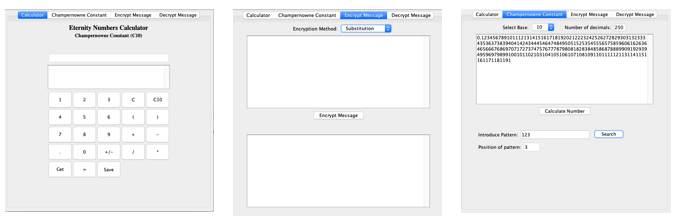
\includegraphics[width=0.8\linewidth]{images/views.png}
\caption{Views of the system}
\end{figure}

\item Importance of Persona: knowing the skills of the user modifies the way exceptions and errors should be handled and the implementation of the system. It is the first time that the concept of persona is studied for a course.\newline



\end{itemize}
\end{block}
%------------------------------------------------






\end{column} % End of column 2

\begin{column}{\onecolwid} 

\begin{block}{Critical Decisions}
\begin{itemize}

\item Selection of graphical over textual interface: the use of a textual interface required more helping features, for the user since the procedure for accessing the operations was not self explanatory. Additionally, the textual interface required less decimals since the information is more difficult to read from the console than from the graphical interface. Even though the potential users have the necessary skills to use a console application the interviewees mentioned that they prefer an application that they can use from the mobile phone or their computer and that provides graphical features. \newline

\item Implementation of the encryption and decryption user stories: the encryption and decryption of messages was prioritize since it was mentioned by one of the interviewees as main application of the number. Additionally, the other interviewee expressed that he would not use the Champernowne Constant for its randomness and that more specialized tools bring a lot of functionalities related to graphs.\newline

\item Calculation of the number by construction and not by the formula: the Champernowne Constant can be constructed by concatenating a sequence of integers in String format or by following a mathematic formula. The construction was selected over the formula because of the big number of decimals necessary for the encryption of messages and pattern formation, high accuracy and precision was required and around 300 decimals of the number.\newline

\item Perform two interviews instead of one: the first interviewee was an expert in numbers theory (university professor) and provided a lot of information about the domain; however, he expressed that he would not use the calculator which motivated the second interview (a master student).

\end{itemize}


\end{block}

\end{column} % End of column 3

\begin{column}{\sepwid}\end{column} % Empty spacer column

\begin{column}{\onecolwid} % The third column

%----------------------------------------------------------------------------------------
%	CONCLUSION
%----------------------------------------------------------------------------------------

\begin{block}{Challenges and Difficulties}

\begin{itemize}
\item Implementation of the user stories without using built-in functions in Java.\newline
\item Determine an appropriate number of decimals for the mathematical operations.\newline
\item Validation of user error in the inputs to the system. This includes the mathematical expression validation for the basic calculator.\newline
\item Understanding of ciphers implementation for decryption and encryption of messages.\newline
\item Finding people to interview that have knowledge of the applications of the Champernowne Constant. \newline

\begin{figure}

\includegraphics[width=0.3\linewidth]{images/champ.png}
\caption{Champernowne Constant}
\end{figure}

\end{itemize}
\end{block}

\begin{block}{References}

\nocite{*} % Insert publications even if they are not cited in the poster
\small{\bibliographystyle{unsrt}
\bibliography{sample}\vspace{0.75in}}

\end{block}

\setbeamercolor{block alerted title}{fg=black,bg=dorado} % Change the alert block title colors
\setbeamercolor{block alerted body}{fg=black,bg=white} % Change the alert block body colors

\begin{alertblock}{Project Repository Link}
https://github.com/NellybettIrahola/SOEN6481-Calculator
\end{alertblock}

%----------------------------------------------------------------------------------------

\end{column} % End of the third column

\end{columns} % End of all the columns in the poster

\end{frame} % End of the enclosing frame

\end{document}
